\section{HÌNH THANG - HÌNH THANG CÂN}
\subsubsection{Kiến thức trọng tâm }
\subsection{Hình thang}
		\immini{
		\begin{boxdn}
			Hình thang là tứ giác có hai cạnh đối song song.
			\end{boxdn}}{
			\begin{tikzpicture}[line join=round, line cap=round,font=\normalsize,>=stealth,scale=1]
				\path 
				(0,0) coordinate (D)
				(D)--++(70:3) coordinate (A)
				(A)--++(0:2.5) coordinate (B)
				(D)--++(0:6) coordinate (C)
				($(D)!(A)!(C)$) coordinate (H)
				;
				\draw (A)--(B)--(C)--(D)--cycle
				(A)--(H);
				\path (H) pic[draw,angle radius=5pt,angle eccentricity=2]{right angle=D--H--A};
				\foreach \x/\g in {A/135,B/45,C/0,D/180,H/-90}{
					\draw[fill=black] (\x) circle (0.05)+(\g:0.3) node {$\x$};
				};
				\draw (A)--(B) node[midway, sloped, above]{đáy nhỏ};
				\draw (B)--(C) node[midway, sloped, above]{cạnh bên};
				\draw (D)--(A) node[midway, sloped, above]{cạnh bên};
				\draw (D)--(C) node[midway, sloped, above]{đáy lớn};
				\draw (H)--(A) node[midway, sloped, below]{đường cao};
			\end{tikzpicture}
		}
\subsection{Hình thang vuông}
		\immini{
		\begin{boxdn}
			Hình thang vuông là hình thang có một góc vuông.
	\end{boxdn}}{
		\begin{tikzpicture}[line join=round, line cap=round,font=\normalsize,>=stealth,scale=1]
			\path 
			(0,0) coordinate (D)
			(D)--++(90:3) coordinate (A)
			(A)--++(0:2.5) coordinate (B)
			(D)--++(0:5) coordinate (C)
			;
			\draw (A)--(B)--(C)--(D)--cycle;
			\path (C) pic[draw,angle radius=5pt,angle eccentricity=2]{right angle=C--D--A};
			\foreach \x/\g in {A/135,B/45,C/0,D/180}{
				\draw[fill=black] (\x) circle (0.05)+(\g:0.3) node {$\x$};
			};
		\end{tikzpicture}
	}
\subsection{Hình thang cân} 
		\immini{
		\begin{boxdn}
			Hình thang cân là hình thang có hai góc kề một đáy bằng nhau.
	\end{boxdn}}{
		\begin{tikzpicture}[line join=round, line cap=round,font=\normalsize,>=stealth,scale=1]
			\path 
			(0,0) coordinate (D)
			(D)--++(70:3) coordinate (A)
			(D)--++(0:5) coordinate (C)
			(C)--++(110:3) coordinate (B)
			;
			\draw (A)--(B)--(C)--(D)--cycle;
			\path (D) pic[draw=black, angle radius=5mm] {angle=C--D--A};
			\path (C) pic[draw=black, angle radius=5mm] {angle=B--C--D};
			\path (A) pic[draw=black,double, angle radius=5mm] {angle=D--A--B};
			\path (B) pic[draw=black,double, angle radius=5mm] {angle=A--B--C};
			\foreach \x/\g in {A/135,B/45,C/0,D/180}{
				\draw[fill=black] (\x) circle (0.05)+(\g:0.3) node {$\x$};
			};
		\end{tikzpicture}
	}
\subsection{Tính chất của hình thang cân} 
	\immini{
		\begin{boxdn}
			Trong hình thang cân
			\begin{itemize}
				\item Hai cạnh bên bằng nhau: $AD=BC$.
				\item Hai đường chéo bằng nhau: $AC=BD$.
				\item Hai góc đối bù nhau: $\widehat{A}+\widehat{C}=\widehat{B}+\widehat{D}=180^\circ$.
		\end{itemize}
		\end{boxdn}
	}{
		\begin{tikzpicture}[line join=round, line cap=round,font=\normalsize,>=stealth,scale=1]
	\path 
	(0,0) coordinate (D)
	(D)--++(70:3) coordinate (A)
	(D)--++(0:5) coordinate (C)
	(C)--++(110:3) coordinate (B)
	;
	\draw (A)--(B)--(C)--(D)--cycle
	(A)--(C) (B)--(D);
	\path (D) pic[draw=black, angle radius=5mm] {angle=C--D--A};
	\path (C) pic[draw=black, angle radius=5mm] {angle=B--C--D};
	\path (A) pic[draw=black,double, angle radius=5mm] {angle=D--A--B};
	\path (B) pic[draw=black,double, angle radius=5mm] {angle=A--B--C};
	\path (A)--(D) node[midway,sloped]{|};
	\path (B)--(C) node[midway,sloped]{|};
	\foreach \x/\g in {A/135,B/45,C/0,D/180}{
		\draw[fill=black] (\x) circle (0.05)+(\g:0.3) node {$\x$};
	};
\end{tikzpicture}
	}
\subsection{Dấu hiệu nhận biết hình thang cân}
	\begin{boxdn}
		\begin{itemize}
			\item Hình thang có hai góc kề một đáy bằng nhau là hình thang cân.
			\item Hình thang có hai đường chéo bằng nhau là hình thang cân. 
		\end{itemize}
	\end{boxdn}
\begin{dang}{Xác định các yếu tố hình thang}
\end{dang}
%%=======Câu [số câu]=======%%
\begin{vd} %[9-EX-DeCuongToan9-L2-Nguyễn Tấn Tài]%[8H2N3-1]
	Tìm các đoạn thẳng bằng nhau có trên hình thang cân $EFGH$ ($EF\parallel HG$).
	\loigiai{
		\immini{
			Hình thang cân $EFGH$ có hai đáy là $EF$ và $HG$ nên có
			\begin{itemize}
				\item Hai cạnh bên bằng nhau $EH=FG$;
				\item Hai đường chéo bằng nhau $EG=HF$.
			\end{itemize}
			
		}{
			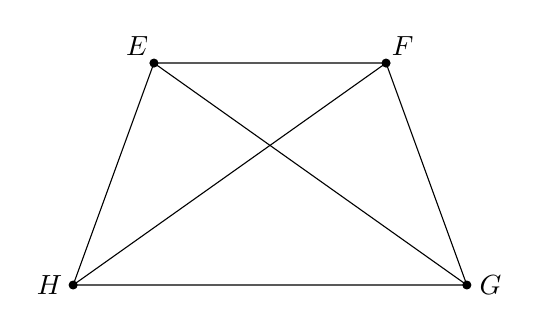
\begin{tikzpicture}[line join=round, line cap=round,font=\normalsize,>=stealth,scale=1]
				\path 
				(0,0) coordinate (H)
				(H)--++(70:3) coordinate (E)
				(H)--++(0:5) coordinate (G)
				(G)--++(110:3) coordinate (F)
				;
				\draw (E)--(F)--(G)--(H)--cycle (H)--(F) (E)--(G);
				\foreach \x/\g in {E/135,F/45,G/0,H/180}{
					\draw[fill=black] (\x) circle (0.05)+(\g:0.3) node {$\x$};
				};
			\end{tikzpicture}
		}
	}
\end{vd}

\begin{dang}{Tính số đo góc}
	{\textbf{Phương pháp giải}
		\begin{itemize}
			\item	Vận dụng các tính chất về góc tạo bởi một đường thẳng cắt hai đường thẳng song song.
			\item	Vận dụng tính chất trong hình thang cân : hai góc kề một đáy bằng nhau, hai góc đối bù nhau.
		\end{itemize}
	}	
\end{dang}
\begin{vd}%[9-EX-DeCuongToan9-L2-Nguyễn Tấn Tài]%[8H2H3-2]	
	Cho hình thang $ABCD$ ($AB \parallel  CD$). Tìm các số đo $x$ và $y$ trong các hình vẽ sau:
	\begin{center}
		\begin{tikzpicture}[line join=round, line cap=round,font=\normalsize,>=stealth,scale=1]
			\path 
			(0,0) coordinate (D)
			(D)--++(80:2.5) coordinate (A)
			(A)--++(0:2) coordinate (B)
			(D)--++(0:4) coordinate (C)
			;
			\draw (A)--(B)--(C)--(D)--cycle;
			\path (A) pic["$100^\circ$",angle eccentricity=1.2] {angle=D--A--B};
			\path (D) pic["$x$",angle eccentricity=1.2] {angle=C--D--A};
			\path (C) pic["$y$",angle eccentricity=1.2] {angle=B--C--D};
			\path (B) pic["$120^\circ$",angle eccentricity=1.2] {angle=A--B--C};
			\foreach \x/\g in {A/135,B/45,C/0,D/180}{
				\draw[fill=black] (\x) circle (0.05)+(\g:0.3) node {$\x$};
			};
			\node at (2,-.5) {a)};
		\end{tikzpicture}
		\begin{tikzpicture}[line join=round, line cap=round,font=\normalsize,>=stealth,scale=1]
			\path 
			(0,0) coordinate (D)
			(D)--++(90:2.3) coordinate (A)
			(A)--++(0:2) coordinate (B)
			(D)--++(0:4) coordinate (C)
			;
			\draw (A)--(B)--(C)--(D)--cycle;
			\path (A) pic["$x$",angle eccentricity=1.2] {angle=D--A--B};
			\path (B) pic["$y$",angle eccentricity=1.2] {angle=A--B--C};
			\path (C) pic["$45^\circ$",angle eccentricity=1.2] {angle=B--C--D};
			\path (C) pic[draw,angle radius=5pt,angle eccentricity=2]{right angle=C--D--A};
			\foreach \x/\g in {A/135,B/45,C/0,D/180}{
				\draw[fill=black] (\x) circle (0.05)+(\g:0.3) node {$\x$};
			};
			\node at (2,-.5) {b)};
		\end{tikzpicture}
		\begin{tikzpicture}[line join=round, line cap=round,font=\normalsize,>=stealth,scale=1]
			\path 
			(0,0) coordinate (D)
			(D)--++(70:2.2) coordinate (A)
			(D)--++(0:4) coordinate (C)
			(C)--++(110:2.2) coordinate (B)
			;
			\draw (A)--(B)--(C)--(D)--cycle;
			\path (A) pic["$x$",angle eccentricity=1.2] {angle=D--A--B};
			\path (D) pic["$70^\circ$",angle eccentricity=1.2] {angle=C--D--A};
			\path (C) pic["$y$",angle eccentricity=1.2] {angle=B--C--D};
			\path (B) pic["$130^\circ$",angle eccentricity=1.2] {angle=A--B--C};
			\foreach \x/\g in {A/135,B/45,C/0,D/180}{
				\draw[fill=black] (\x) circle (0.05)+(\g:0.3) node {$\x$};
			};
			\node at (2,-.5) {c)};
		\end{tikzpicture}
	\end{center}
	\loigiai{
		\begin{center}
			\begin{tikzpicture}[line join=round, line cap=round,font=\normalsize,>=stealth,scale=1]
				\path 
				(0,0) coordinate (D)
				(D)--++(80:2.5) coordinate (A)
				(A)--++(0:2) coordinate (B)
				(D)--++(0:4) coordinate (C)
				;
				\draw (A)--(B)--(C)--(D)--cycle;
				\path (A) pic["$100^\circ$",angle eccentricity=1.2] {angle=D--A--B};
				\path (D) pic["$x$",angle eccentricity=1.2] {angle=C--D--A};
				\path (C) pic["$y$",angle eccentricity=1.2] {angle=B--C--D};
				\path (B) pic["$120^\circ$",angle eccentricity=1.2] {angle=A--B--C};
				\foreach \x/\g in {A/135,B/45,C/0,D/180}{
					\draw[fill=black] (\x) circle (0.05)+(\g:0.3) node {$\x$};
				};
				\node at (2,-.5) {a)};
			\end{tikzpicture}
			\begin{tikzpicture}[line join=round, line cap=round,font=\normalsize,>=stealth,scale=1]
				\path 
				(0,0) coordinate (D)
				(D)--++(90:2.3) coordinate (A)
				(A)--++(0:2) coordinate (B)
				(D)--++(0:4) coordinate (C)
				;
				\draw (A)--(B)--(C)--(D)--cycle;
				\path (A) pic["$x$",angle eccentricity=1.2] {angle=D--A--B};
				\path (B) pic["$y$",angle eccentricity=1.2] {angle=A--B--C};
				\path (C) pic["$45^\circ$",angle eccentricity=1.2] {angle=B--C--D};
				\path (C) pic[draw,angle radius=5pt,angle eccentricity=2]{right angle=C--D--A};
				\foreach \x/\g in {A/135,B/45,C/0,D/180}{
					\draw[fill=black] (\x) circle (0.05)+(\g:0.3) node {$\x$};
				};
				\node at (2,-.5) {b)};
			\end{tikzpicture}
			\begin{tikzpicture}[line join=round, line cap=round,font=\normalsize,>=stealth,scale=1]
				\path 
				(0,0) coordinate (D)
				(D)--++(70:2.2) coordinate (A)
				(D)--++(0:4) coordinate (C)
				(C)--++(110:2.2) coordinate (B)
				;
				\draw (A)--(B)--(C)--(D)--cycle;
				\path (A) pic["$x$",angle eccentricity=1.2] {angle=D--A--B};
				\path (D) pic["$70^\circ$",angle eccentricity=1.2] {angle=C--D--A};
				\path (C) pic["$y$",angle eccentricity=1.2] {angle=B--C--D};
				\path (B) pic["$130^\circ$",angle eccentricity=1.2] {angle=A--B--C};
				\foreach \x/\g in {A/135,B/45,C/0,D/180}{
					\draw[fill=black] (\x) circle (0.05)+(\g:0.3) node {$\x$};
				};
				\node at (2,-.5) {c)};
			\end{tikzpicture}
		\end{center}
		\begin{enumerate}
			\item	Vì $AB\parallel  CD$ nên 
			\begin{eqnarray*}
				\widehat{A}+\widehat{D}&=&180^\circ \\
				100^\circ+x&=&180^\circ \\
				x&=&80^\circ.
			\end{eqnarray*}
			\begin{eqnarray*}
				\widehat{B}+\widehat{C}&=&180^\circ \\
				120^\circ+y&=&180^\circ \\
				y&=&60^\circ.
			\end{eqnarray*}
			
			\item	Vì $AB\parallel CD$ nên 
			\begin{eqnarray*}
				\widehat{A}+\widehat{D} &=& 180^\circ \\
				x+90^\circ &=& 180^\circ \\
				x &=& 90^\circ.
			\end{eqnarray*}
			
			\begin{eqnarray*}
				\widehat{B}+\widehat{C} &=& 180^\circ \\
				y+45^\circ &=& 180^\circ \\
				y &=& 135^\circ.
			\end{eqnarray*}
			
			\item	Vì $AB\parallel CD$ nên 
			\begin{eqnarray*}
				\widehat{A}+\widehat{D} &=& 180^\circ \\
				x+70^\circ &=& 180^\circ \\
				x &=& 110^\circ.
			\end{eqnarray*}
			
			\begin{eqnarray*}
				\widehat{B}+\widehat{C} &=& 180^\circ \\
				130^\circ+y &=& 180^\circ \\
				y &=& 50^\circ.
			\end{eqnarray*}
			
		\end{enumerate}	
	}
\end{vd}
\begin{dang}{Tính độ dài cạnh bên, đường cao, hai đường chéo}
	
\end{dang}
\begin{vd}%[9-EX-DeCuongToan9-L2-Nguyễn Tấn Tài]%[8H2H3-2]	
	Hình thang cân $ABCD$ có đáy nhỏ $AB=10$ cm, đáy lớn $CD=20$ cm và đường cao $AH=12$ cm. Tính độ dài cạnh bên.
	\loigiai{
		\immini{
			Vẽ $BK \perp CD$.\\
			Xét $\triangle ADH$ và $\triangle BCK$, ta có\\
			$AD=BC$ (cạnh bên hình thang cân);\\
			$\widehat{D}=\widehat{C}$ (góc kề cạnh đáy của hình thang cân);\\
			Suy ra $\triangle ADH=\triangle BCK$(cạnh huyền, góc nhọn).\\
			Suy ra $HD=KC=\dfrac{CD-HK}{2}=\dfrac{20-10}{2}=5$ cm\\
			Xét $ADH$ vuông tại $H$, ta có
			\begin{eqnarray*}
				AD^2 &=& AH^2+HD^2 \quad \text{(Định lý Pythagore)} \\
				AD^2&=& 12^2+5^2\\
				AD^2&=&144+25\\
				AD^2&=&169 \\
				AD &=& \sqrt{169}=13\,\text{cm}.
			\end{eqnarray*}
			
			}{
			\begin{tikzpicture}[line join=round, line cap=round,font=\normalsize,>=stealth,scale=1]
				\path 
				(0,0) coordinate (D)
				(D)--++(70:3) coordinate (A)
				(D)--++(0:5) coordinate (C)
				(C)--++(110:3) coordinate (B)
				($(D)!(A)!(C)$) coordinate (H)
				($(D)!(B)!(C)$) coordinate (K)
				;
				\draw (A)--(B)--(C)--(D)--cycle (A)--(H) (B)--(K);
				\path (H) pic[draw,angle radius=5pt,angle eccentricity=2]{right angle=D--H--A};
				\path (K) pic[draw,angle radius=5pt,angle eccentricity=2]{right angle=B--K--C};
				\foreach \x/\g in {A/135,B/45,C/0,D/180,B/45,H/-90,K/-90}{
					\draw[fill=black] (\x) circle (0.05)+(\g:0.3) node {$\x$};
				};
			\end{tikzpicture}
		}
	}
\end{vd}
\begin{dang}{Chứng minh tứ giác là hình thang, hình thang vuông, hình thang cân}

\end{dang}
\begin{vd}%[9-EX-DeCuongToan9-L2-Nguyễn Tấn Tài]%[8H2H3-3]
	Tứ giác $ABCD$ có $\widehat{A}+\widehat{D}=\widehat{B}+\widehat{C}$. Chứng minh rằng tứ giác $ABCD$ là hình thang.
	\loigiai{
		\immini{
			Ta có $\widehat{A}+\widehat{D}+\widehat{B}+\widehat{C}=360^\circ$\\
			mà $\widehat{A}+\widehat{D}=\widehat{B}+\widehat{C}$ nên $2(\widehat{A} +\widehat{D})=360^\circ $. \\
			nên $\widehat{A}+\widehat{D}=180^\circ $.\\
			Suy ra $AB\parallel CD$ (vì có cặp góc trong cùng phía bù nhau).\\
			Do đó tứ giác $ABCD$ là hình thang.}{
			\begin{tikzpicture}[line join=round, line cap=round,font=\normalsize,>=stealth,scale=1]
				\path 
				(0,0) coordinate (D)
				(D)--++(70:3) coordinate (A)
				(A)--++(0:2.5) coordinate (B)
				(D)--++(0:6) coordinate (C)
				;
				\draw (A)--(B)--(C)--(D)--cycle;
				\foreach \x/\g in {A/135,B/45,C/0,D/180}{
					\draw[fill=black] (\x) circle (0.05)+(\g:0.3) node {$\x$};
				};
			\end{tikzpicture}
		}
	}
\end{vd}

\begin{vd}%[9-EX-DeCuongToan9-L2-Nguyễn Tấn Tài]%[8H2H3-3]
	Cho tam giác $ABC$ cân tại $A$. Trên tia đối của tia $AB$ lấy điểm $M$, trên tia đối của tia $AC$ lấy điểm $N$ sao cho $AM=AN$. Chứng minh rằng tứ giác $MNBC$ là hình thang cân.
	\loigiai{
		\immini{
			$\triangle ABC$ cân tai $A$ suy ra $\widehat{ABC}=\dfrac{180^\circ -\widehat{BAC}}{2}$.\\
			$\triangle AMN$ cân tai $A$ suy ra $\widehat{AMN}=\dfrac{180^\circ -\widehat{MAN}}{2}$.\\
			Mặt khác $\widehat{BAC}=\widehat{MAN}$ nên $\widehat{ABC}=\widehat{AMN}$.\\
			Suy ra $MN \parallel BC$ nên tứ giác $MNBC$ là hình thang.\\
			Ta có $AB=AC$; $AM=AN$.\\
			Suy ra $AB+AM=AC+AN$ hay $MB=NC$.\\
			Hình thang $MNBC$ có hai đường chéo bằng nhau nên là hình thang cân.}{
			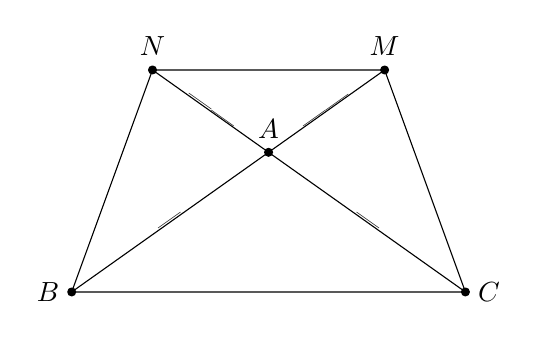
\begin{tikzpicture}[line join=round, line cap=round,font=\normalsize,>=stealth,scale=1]
				\path 
				(0,0) coordinate (B)
				(B)--++(70:3) coordinate (N)
				(B)--++(0:5) coordinate (C)
				(C)--++(110:3) coordinate (M)
				(intersection of B--M and C--N) coordinate (A)
				;
				\draw (B)--(C)--(M)--(N)--cycle
				(N)--(C) (B)--(M);
				\path (A)--(B) node[midway,sloped]{|};
				\path (A)--(C) node[midway,sloped]{|};
				\path (A)--(M) node[midway,sloped]{||};
				\path (A)--(N) node[midway,sloped]{||};
				\foreach \x/\g in {A/90,B/180,C/0,M/90,N/90}{
					\draw[fill=black] (\x) circle (0.05)+(\g:0.3) node {$\x$};
				};
			\end{tikzpicture}
		}
	}
\end{vd}

\begin{vd}%[9-EX-DeCuongToan9-L2-Nguyễn Tấn Tài]%[8H2H3-3]
	Tứ giác $ABCD$ có $\widehat{A}=\widehat{B}$, $\widehat{C}=\widehat{D}$. Chứng minh rằng tứ giác $ABCD$ là hình thang cân.
	\loigiai{
		\immini{
			Ta có $\widehat{A}+ \widehat{B}+\widehat{C}+\widehat{D}=360^\circ$ \\
			hay $2\widehat{A}+2\widehat{D}=360^\circ$\\
			Suy ra $\widehat{A}+ \widehat{D}=180^\circ$.\\
			Do đó $AB\parallel CD$.\\
			Vậy tứ giác $ABCD$ là hình thang cân.}{
			\begin{tikzpicture}[line join=round, line cap=round,font=\normalsize,>=stealth,scale=1]
				\path 
				(0,0) coordinate (D)
				(D)--++(70:3) coordinate (A)
				(D)--++(0:5) coordinate (C)
				(C)--++(110:3) coordinate (B)
				;
				\draw (A)--(B)--(C)--(D)--cycle;
				\path (D) pic[draw=black, angle radius=5mm] {angle=C--D--A};
				\path (C) pic[draw=black, angle radius=5mm] {angle=B--C--D};
				\path (A) pic[draw=black,double, angle radius=5mm] {angle=D--A--B};
				\path (B) pic[draw=black,double, angle radius=5mm] {angle=A--B--C};
				\foreach \x/\g in {A/135,B/45,C/0,D/180}{
					\draw[fill=black] (\x) circle (0.05)+(\g:0.3) node {$\x$};
				};
			\end{tikzpicture}
		}
	}
\end{vd} 
\subsubsection{Bài tập}
\begin{bt}%[9-EX-DeCuongToan9-L2-Nguyễn Tấn Tài]%[8H2H3-2]
	Tìm $x$ và $y$ ở các hình sau
	\begin{center}
		\begin{tikzpicture}[scale=0.9]
			\def\a{4}
			\path (	0,0) coordinate (D)--+(\a,0) coordinate (C)
			($(C)!0.1!-40:(D)$) coordinate (x)
			($(C)!6!(x)$) coordinate (B)
			($(D)+(B)-(C)$) coordinate (y)
			($(B)!1/3!(y)$) coordinate (A)
			;
			\path pic["\scriptsize$x$", angle eccentricity=1]{angle=B--C--D};
			\path pic["\scriptsize$140^\circ$"]{angle=A--B--C};
			\draw (D)--(C)--(B)--(A)--cycle ($(D)!.5!(C)$)node[below]{$AB\parallel CD$}
			;
			\foreach \t/\g in {D/180,C/0,B/0,A/180}{
				\draw[fill=white] (\t) circle (1pt) node[shift={(\g:7pt)},font=\scriptsize]{$ \t $};
			}
			\node[below] at (current bounding box.south){$a)$};  	
		\end{tikzpicture}
		\begin{tikzpicture}[scale=0.9]
			\def\a{2}
			\path (	0,0) coordinate (M)--+(0,\a) coordinate (Q)
			($(Q)!0.1!60:(M)$) coordinate (x)
			($(M)!1!-120:(Q)$) coordinate (y)
			($(M)!0.8!(y)$) coordinate (N)
			($(N)!0.1!70:(y)$) coordinate (y')
			(intersection of Q--x and N--y') coordinate (P)
			
			;
			\path pic["\scriptsize$x$", angle eccentricity=1]{angle=N--M--Q};
			\path pic["\scriptsize$y$", angle eccentricity=1]{angle=Q--P--N};
			\path pic["\scriptsize$60^\circ$", angle eccentricity=1]{angle=M--Q--P};
			\path pic["\scriptsize$70^\circ$", angle eccentricity=1]{angle=y--N--P};
			\draw (Q)--(M)--(y) (N)--(P)--(Q) (N)node[below=3mm]{$MN\parallel PQ$}
			;
			\foreach \t/\g in {M/180,Q/90,N/-90,P/0}{
				\draw[fill=white] (\t) circle (1pt) node[shift={(\g:7pt)},font=\scriptsize]{$ \t $};
			}
			\node[below] at (current bounding box.south){$b)$};  	
		\end{tikzpicture}	
		\begin{tikzpicture}[scale=1]
			\def\a{3}
			\path (	0,0) coordinate (I)--+(\a,0) coordinate (K)
			($(I)!0.1!36:(K)$) coordinate (x)
			($(K)!0.1!-72:(I)$) coordinate (y)
			($(I)!6!(x)$) coordinate (H)
			($(K)+(H)-(I)$) coordinate (y')
			(intersection of H--y' and K--y) coordinate (G)
			
			;
			\path pic["\scriptsize$x$", angle eccentricity=1]{angle=K--I--H};
			\path pic["\scriptsize$2x$", angle eccentricity=0.6]{angle=G--K--I};
			\path pic["\scriptsize$3x$", angle eccentricity=0.5]{angle=H--G--K};
			\path pic["\scriptsize$4x$", angle eccentricity=0.5]{angle=I--H--G};
			\draw (I)--(K)--(G)--(H)--cycle ($(I)!.5!(K)$)node[below]{$HG\parallel KI$}
			;
			\foreach \t/\g in {I/180,K/0,H/180,G/0}{
				\draw[fill=white] (\t) circle (1pt) node[shift={(\g:7pt)},font=\scriptsize]{$ \t $};
			}
			\node[below] at (current bounding box.south){$c)$};  	
		\end{tikzpicture}
		\begin{tikzpicture}[scale=0.65]
			\def\a{3}
			\path (	0,0) coordinate (S)--+(\a,0) coordinate (T)
			($(S)!0.5!90:(T)$) coordinate (V)
			($(T)!1!-90:(S)$) coordinate (U)
			;
			\path pic["\scriptsize$x$", angle eccentricity=0.6]{angle=V--U--T};
			\path pic["\scriptsize$2x$", angle eccentricity=0.6]{angle=S--V--U};
			\foreach \x/\y/\z in {V/S/T,U/T/S}{
				\path pic[draw,angle radius=5pt]{right angle=\x--\y--\z};
			}
			\draw (S)--(T)--(U)--(V)--cycle
			;
			\foreach \t/\g in {S/180,T/0,V/180,U/0}{
				\draw[fill=white] (\t) circle (1pt) node[shift={(\g:7pt)},font=\scriptsize]{$ \t $};
			}
			\node[below] at (current bounding box.south){$d)$};  	
		\end{tikzpicture}
	\end{center}
	\loigiai{
		\begin{enumerate}
			\item 
			Vì $AB\parallel  CD$ nên 
			\begin{eqnarray*}
				\widehat{B}+\widehat{C}&=&180^\circ \\
				140^\circ+x&=&180^\circ \\
				x&=&40^\circ.
			\end{eqnarray*}
			\item 
			Vì $MN\parallel  PQ$ nên 
			\begin{eqnarray*}
				\widehat{M}+\widehat{Q}&=&180^\circ \\
				x+60^\circ&=&180^\circ \\
				x&=&120^\circ.
			\end{eqnarray*}
			\begin{eqnarray*}
				y&=&70^\circ \text{(so le trong)}.
			\end{eqnarray*}
			\item Ta có
			\begin{eqnarray*}
				\widehat{I}+\widehat{K}+\widehat{G}+\widehat{H}&=&360^\circ \quad \text{(Tổng các góc của tứ giác)} \\
				x+2x+3x+4x&=&360^\circ \\
				10x&=&360^\circ\\
				x&=&36^\circ.
			\end{eqnarray*}
			\item 
			Ta có
			\begin{eqnarray*}
				\widehat{U}+\widehat{V}+\widehat{S}+\widehat{T}&=&360^\circ \quad \text{(Tổng các góc của tứ giác)} \\
				x+2x+90+90&=&360^\circ \\
				3x&=&180^\circ\\
				x&=&60^\circ.
			\end{eqnarray*}
		\end{enumerate}	
	}
\end{bt}
\begin{bt}%[9-EX-DeCuongToan9-L2-Nguyễn Tấn Tài]%[8H2H3-2]
	Cho hình thang $ABCD$ ($AB\parallel CD$) có $\widehat{B}-\widehat{C}=40^\circ$; $\widehat{C}-\widehat{D}=20^\circ$. Tính các góc của hình thang?
	\loigiai{
		\immini{
			Vì $AB\parallel CD$ nên $\widehat{B}+\widehat{C}=180^\circ$.\\
			Mặt khác $\widehat{B}-\widehat{C}=40^\circ$.\\
			Suy ra 
			$\widehat{B}=(180^\circ +40^\circ):2=110^\circ$;\\
			$\widehat{C}=180^\circ -110^\circ=70^\circ$.\\
			Ta lại có 
			$\widehat{C}-\widehat{D}=20^\circ$ nên $70^\circ-\widehat{D}=20^\circ$.\\
			Suy ra $\widehat{D}=50^\circ$.\\
			Do đó $\widehat{A}=180^\circ-\widehat{D}=180^\circ -50^\circ=130^\circ$.
		}{
			\begin{tikzpicture}[line join=round, line cap=round,font=\normalsize,>=stealth,scale=1]
				\path 
				(0,0) coordinate (D)
				(D)--++(70:3) coordinate (A)
				(A)--++(0:2.5) coordinate (B)
				(D)--++(0:6) coordinate (C)
				;
				\draw (A)--(B)--(C)--(D)--cycle;
				\foreach \x/\g in {A/135,B/45,C/0,D/180}{
					\draw[fill=black] (\x) circle (0.05)+(\g:0.3) node {$\x$};
				};
			\end{tikzpicture}
		}
	}
\end{bt}
\begin{bt}%[9-EX-DeCuongToan9-L2-Nguyễn Tấn Tài]%[8H2H3-2]
	Cho hình thang cân $ABCD$ ($AB\parallel CD$) có $A=120^\circ$. Tính số đo các góc còn lại?
	\loigiai{
	\immini{
			Trong hình thang cân, hai góc kề một đáy bằng nhau nên\\ $\widehat{B}=\widehat{A}=120^\circ$.\\
			Trong hình thang cân, hai góc đối bù nhau nên\\ $\widehat{A}+\widehat{C}=180^\circ$.\\
			Suy ra $\widehat{C}=180^\circ-120^\circ=60^\circ$.\\
			Do đó $\widehat{D}=\widehat{C}=60^\circ$.
	}{
	\begin{tikzpicture}[line join=round, line cap=round,font=\normalsize,>=stealth,scale=1]
	\path 
	(0,0) coordinate (D)
	(D)--++(70:3) coordinate (A)
	(D)--++(0:5) coordinate (C)
	(C)--++(110:3) coordinate (B)
	;
	\draw (A)--(B)--(C)--(D)--cycle;
	\path (D) pic[draw=black, angle radius=5mm] {angle=C--D--A};
	\path (C) pic[draw=black, angle radius=5mm] {angle=B--C--D};
	\path (A) pic[draw=black,double, angle radius=5mm] {angle=D--A--B};
	\path (B) pic[draw=black,double, angle radius=5mm] {angle=A--B--C};
	\foreach \x/\g in {A/135,B/45,C/0,D/180}{
		\draw[fill=black] (\x) circle (0.05)+(\g:0.3) node {$\x$};
	};
\end{tikzpicture}
	}
	}
\end{bt}
\begin{bt}%[9-EX-DeCuongToan9-L2-Nguyễn Tấn Tài]%[8H2H3-3]
	Cho hình thang cân $ABCD$ ($AB\parallel CD$). Chứng minh rằng $\widehat{CAD}=\widehat{DBC}$.
	\loigiai{
		\immini{
			$\triangle CAD$ và $\triangle DBC$ có\\
			$AD=BC$ (hai cạnh bên),\\
			$\widehat{ADC}=\widehat{BCD}$ (hai góc kề đáy),\\
			$CD$ chung.\\
			Vậy $\triangle CAD=\triangle DBC$ (c.g.c).\\
			Suy ra $\widehat{CAD}=\widehat{DBC}$.}{
			\begin{tikzpicture}[line join=round, line cap=round,font=\normalsize,>=stealth,scale=1]
				\path 
				(0,0) coordinate (D)
				(D)--++(70:3) coordinate (A)
				(D)--++(0:5) coordinate (C)
				(C)--++(110:3) coordinate (B)
				;
				\draw (A)--(B)--(C)--(D)--cycle
				(A)--(C) (B)--(D);
				\path (D) pic[draw=black, angle radius=5mm] {angle=C--D--A};
				\path (C) pic[draw=black, angle radius=5mm] {angle=B--C--D};
				\path (A) pic[draw=black,double, angle radius=5mm] {angle=D--A--B};
				\path (B) pic[draw=black,double, angle radius=5mm] {angle=A--B--C};
				\path (A)--(D) node[midway,sloped]{|};
				\path (B)--(C) node[midway,sloped]{|};
				\foreach \x/\g in {A/135,B/45,C/0,D/180}{
					\draw[fill=black] (\x) circle (0.05)+(\g:0.3) node {$\x$};
				};
			\end{tikzpicture}
		}
	}
\end{bt}
%%=======Câu [số câu]=======%%
\begin{bt}%[9-EX-DeCuongToan9-L2-Nguyễn Tấn Tài]%[8H2H3-2]
	Cho hình thang cân $ABCD$ có $AB\parallel CD$, $AB<CD$. Gọi $H$, $K$ lần lượt là hình chiếu của $A$, $B$ trên đường thẳng $CD$. Chứng minh rằng $DH=CK$.
	\loigiai{
		\immini{
		Xét hai tam giác vuông $ADH$ và $BCK$, ta có\\
		$AD=BC$ (vì $ABCD$ là hình thang cân);\\
		$\widehat{ADH}=\widehat{BCK}$ (vì $ABCD$ là hình thang cân).\\
		Suy ra $\triangle ADH = \triangle BCK$ (cạnh huyền - góc nhọn).\\
		Do đó $DH=CK$ (hai cạnh tương ứng).
		}{
		\begin{tikzpicture}[scale=0.7]
			\def\a{5}
			\path (	0,0) coordinate (D)--+(\a,0) coordinate (C)
			($(D)!0.1!60:(C)$) coordinate (x)
			($(D)!6!(x)$) coordinate (A)
			($(C)!0.1!-60:(D)$) coordinate (y)
			($(C)+(A)-(D)$) coordinate (x')
			(intersection of A--x' and C--y) coordinate (B)
			($(C)!(A)!(D)$) coordinate (H)
			($(C)!(B)!(D)$) coordinate (K)
			;
			\foreach \x/\y/\z in {A/H/C,B/K/C}{
				\path pic[draw,angle radius=5pt]{right angle=\x--\y--\z};
			}
			\draw (D)--(C)--(B)--(A)--cycle (A)--(H) (B)--(K)
			;
			\foreach \t/\g in {D/-90,C/-90,A/90,B/90,H/-90,K/-90}{
				\draw[fill=white] (\t) circle (1pt) node[shift={(\g:7pt)},font=\scriptsize]{$ \t $};
			}
		\end{tikzpicture}
		}
	}
\end{bt}
\begin{bt}%[9-EX-DeCuongToan9-L2-Nguyễn Tấn Tài]%[8H2H3-2]
	Cho hình thang vuông $ABCD$ ($AB\parallel CD$) có $\widehat{D}=90^\circ$; $\widehat{C}=45^\circ$. Biết $AB=2$; $CD=5$. Tính độ dài $AD$.
	\loigiai{
		\immini{
			Kẻ $BK \perp CD$.\\
			Mà $AB\parallel CD$.\\
			Suy ra $BK \perp AB$.\\
			Xét $\triangle ADK$ và $\triangle ABK$ có\\
			$\widehat{ADK}=\widehat{ABK}=90^\circ$;\\
			$AK$ là cạnh chung;\\
			$\widehat{DKA}=\widehat{BAK}$ (so le trong);\\
			Suy ra $\triangle ADK=\triangle ABK$ (cạnh huyền - góc nhọn).\\
			Suy ra $DK=AB=2$ và $AD=BK$(hai cạnh tương ứng).\\
			Do đó $CK=DC-DK=5-2=3$.\\
			$\triangle KBC$ vuông tại $K$ có $\widehat{C}=45^\circ$ nên là tam giác vuông cân.\\
			Do đó $BK=CK=3$.\\
			Vậy $AD=BK=3$.
		}{
			\begin{tikzpicture}[line join=round, line cap=round,font=\normalsize,>=stealth,scale=1]
				\path 
				(0,0) coordinate (D)
				(D)--++(90:3) coordinate (A)
				(A)--++(0:2.5) coordinate (B)
				(D)--++(0:5) coordinate (C)
				($(C)!(B)!(D)$) coordinate (K)
				;
				\draw (A)--(B)--(C)--(D)--cycle (B)--(K);
				\path (C) pic[draw,angle radius=5pt,angle eccentricity=2]{right angle=C--D--A};
				\path (K) pic[draw,angle radius=5pt,angle eccentricity=2]{right angle=D--K--B};
				\foreach \x/\g in {A/135,B/45,C/0,D/180,K/-90}{
					\draw[fill=black] (\x) circle (0.05)+(\g:0.3) node {$\x$};
				};
			\end{tikzpicture}
		}
	}
\end{bt}
%%=====Bài 5
\begin{bt}%[9-EX-DeCuongToan9-L2-Nguyễn Tấn Tài]%[8H2H3-1]
	Tứ giác nào trong các hình sau là hình thang cân?
	\begin{center}
		\begin{tikzpicture}[scale=0.7]
			\def\a{4}
			\path (	0,0) coordinate (K)--+(\a,0) coordinate (I)
			($(K)!0.6!51:(I)$) coordinate (G)
			($(G)+(I)-(K)$) coordinate (H)
			
			;
			\path pic["\scriptsize$51^\circ$", angle eccentricity=1]{angle=I--K--G};
			\path pic["\scriptsize$51^\circ$", angle eccentricity=1]{angle=G--H--I};
			\path pic["\scriptsize$129^\circ$", angle eccentricity=0.7]{angle=K--G--H};
			\path pic["\scriptsize$129^\circ$", angle eccentricity=0.7]{angle=H--I--K};
			
			\draw (I)--(K)--(G)--(H)--cycle;%--(H)--cycle ($(I)!.5!(K)$)node[below]{$HG\parallel KI$}
			;
			\foreach \t/\g in {K/180,I/0,G/180,H/0}{
				\draw[fill=white] (\t) circle (1pt) node[shift={(\g:7pt)},font=\scriptsize]{$ \t $};
			}
			\node[below] at (current bounding box.south){$a)$};  	
		\end{tikzpicture}
		\begin{tikzpicture}[scale=0.7]
			\def\a{4}
			\path (	0,0) coordinate (N)--+(\a,1) coordinate (P)
			($(N)!0.1!75:(P)$) coordinate (x)
			($(P)!0.1!-75:(N)$) coordinate (y)
			($(P)!6!(y)$) coordinate (Q)
			($(N)+(Q)-(P)$) coordinate (x')
			(intersection of N--x and Q--x') coordinate (M)
			
			;
			\path pic["\scriptsize$75^\circ$", angle eccentricity=1]{angle=x'--M--N};
			\path pic["\scriptsize$75^\circ$", angle eccentricity=1]{angle=Q--P--N};
			\path pic["\scriptsize$105^\circ$", angle eccentricity=1]{angle=M--Q--P};
			\draw (N)--(P)--(Q)--(x') (N)--(M);
			;
			\foreach \t/\g in {N/180,P/0,Q/0,M/120}{
				\draw[fill=white] (\t) circle (1pt) node[shift={(\g:7pt)},font=\scriptsize]{$ \t $};
			}
			\node[below] at (current bounding box.south){$b)$};  	
		\end{tikzpicture}
		\begin{tikzpicture}[scale=0.7]
			\def\a{4}
			\path (	0,0) coordinate (A)--+(\a,0) coordinate (B)
			($(A)!0.1!120:(B)$) coordinate (x)
			($(A)!6!(x)$) coordinate (D)
			($(B)!0.1!-120:(A)$) coordinate (y)
			($(B)+(D)-(A)$) coordinate (x')
			(intersection of D--x' and B--y) coordinate (C)
			($(A)!-0.4!(B)$) coordinate (u)
			($(D)!-0.3!(C)$) coordinate (v)
			;
			\path pic["\scriptsize$60^\circ$", angle eccentricity=1]{angle=D--A--u};
			\path pic["\scriptsize$120^\circ$", angle eccentricity=0.8]{angle=v--D--A};
			\draw (v)--(C)--(B)--(A)--(D) (A)--(u) (A)--(C) (B)--(D) ($(A)!.5!(B)$)node[below]{$AC=BD$}
			;
			\foreach \t/\g in {A/-90,B/-90,D/90,C/90}{
				\draw[fill=white] (\t) circle (1pt) node[shift={(\g:7pt)},font=\scriptsize]{$ \t $};
			}
			\node[below] at (current bounding box.south){$c)$};  	
		\end{tikzpicture}
	\end{center}
	\loigiai{
	\begin{enumerate}
		\item Ta thấy hai góc kề một đáy của tứ giác GHIH có số đo là $51^\circ$ và $129^\circ$ không bằng nhau.\\
		Suy ra tứ giác GHIH không phải là hình thang cân.
		\item Ta có 
		\begin{eqnarray*}
			\widehat{Q_1}+\widehat{MQP}&=&180^\circ \text{(hai góc kề bù)}.\\
			\widehat{Q_1}&=&180^\circ-\widehat{MQP}\\
			\widehat{Q_1}&=&180^\circ-105^\circ\\
			\widehat{Q_1}&=&75^\circ.
		\end{eqnarray*}
		Suy ra $\widehat{Q_1}=\widehat{P}=75^\circ$.\\
		Mà hai góc này ở vị trí đồng vị nên $MQ\parallel NP$.\\
		Suy ra tứ giác MNQP có $MQ\parallel NP$ nên là hình thang.\\
		Lại có $\widehat{N}=75^\circ$ (do là góc so le trong với góc ngoài tại đỉnh $M$),\\
		Suy ra $\widehat{N}=\widehat{P}=75^\circ$.\\
		Suy ra hình thang MNQP có hai góc kề một đáy bằng nhau nên là hình thang cân.
		\item Ta có 
		\begin{eqnarray*}
			\widehat{ADC}+\widehat{D_1}&=&180^\circ \quad \text{(hai góc kề bù)}\\
			\widehat{ADC}&=&180^\circ-\widehat{D_1}\\
			\widehat{ADC}&=&180^\circ-120^\circ\\
			\widehat{ADC}&=&60^\circ.
		\end{eqnarray*}
		Suy ra $\widehat{ADC}=\widehat{A_1}=60^\circ$, mà hai góc này ở vị trí so le trong nên $DC\parallel AB$.\\
		Suy ra tứ giác ABCD có $DC\parallel AB$ và $AC=BD$ nên là hình thang cân.
	\end{enumerate}
	}
\end{bt}
%%=======Câu 1=======%%
\begin{bt}%[9-EX-DeCuongToan9-L2-Nguyễn Tấn Tài]%[8H2H3-3]
	Tứ giác $ABCD$ có $\widehat{B}=\widehat{C}$, $\widehat{A}=3\widehat{D}$, $\widehat{D}=45^\circ$. Hãy cho biết dạng của tứ giác $ABCD$.
	\loigiai{
		Ta có $\widehat{D}=45^\circ$, suy ra $\widehat{A}=3\cdot\widehat{D}=135^\circ$.\\
		Mà tổng các góc trong tứ giác bằng $360^\circ$ nên
		\begin{eqnarray*}
			\widehat{A}+\widehat{B}+\widehat{C}+\widehat{D}&=&360^\circ\\
			135^\circ+\widehat{B}+\widehat{C}+45^\circ&=&360^\circ\\
			\widehat{B}+\widehat{C}&=&180^\circ.
		\end{eqnarray*}
		Lại có $\widehat{B}=\widehat{C}$ nên 
		\begin{eqnarray*}
			2\widehat{B}&=&180^\circ\\
			\widehat{B}&=&\widehat{C}=90^\circ.
		\end{eqnarray*}
		Suy ra $AB \parallel CD$.\\
		Tứ giác $ABCD$ có một cặp cạnh đối song song và $\widehat{B}=90^\circ$ nên $ABCD$ là hình thang vuông.
	}
\end{bt}
%%=====Bài 2
\begin{bt}%[9-EX-DeCuongToan9-L2-Nguyễn Tấn Tài]%[8H2H3-3]
	Cho tứ giác $ABCD$ có $AB=AD$, $BD$ là tia phân giác của góc $B$. Chứng minh rằng $ABCD$ là hình thang.
	\loigiai{
		\immini{
			Ta có $AB=AD\Rightarrow \triangle ABD$ cân tại $A$\\
			Suy ra $\widehat{ABD}=\widehat{ADB}$.\\
			Mà $\widehat{ABD}=\widehat{DBC}$ (do $BD$ là tia phân giác $\widehat{ABC}$).\\
			Suy ra $\widehat{ADB}=\widehat{DBC}$ (hai góc này ở vị trí so le trong).\\
			Do đó $AD\parallel BC$.\\
			Vậy $ABCD$ là hình thang.
		}	
		{
			\begin{tikzpicture}[scale=1]
				\def\a{4}
				\path (	0,0) coordinate (B)--+(\a,0) coordinate (C)
				($(B)!0.1!40:(C)$) coordinate (x)
				($(B)!6!(x)$) coordinate (A)
				($(A)!1!140:(B)$) coordinate (D)
				;
				\foreach \x/\y/\z in {C/B/D,A/D/B}{
					\path pic[draw,angle radius=12pt, double]{angle=\x--\y--\z};
					\path pic[ angle eccentricity=2,draw,angle radius=10pt, double]{angle=D--B--A};
				}
				\draw (D)--(C)--(B)--(A)--cycle  (B)--(D)
				;
				\foreach \x/\y in {A/B,A/D}{
					\path (\x)--(\y) node[midway,sloped]{\tikz{\draw (-90:3pt)--(90:3pt)
							[shift={(0.65pt,0)}](-90:3pt)--(90:3pt)
							[shift={(0.65pt,0)}](-90:3pt)--(90:3pt);}};
				}
				\foreach \t/\g in {B/180,C/0,D/0,A/180}{
					\draw[fill=white] (\t) circle (1pt) node[shift={(\g:7pt)},font=\scriptsize]{$ \t $};
				}
			\end{tikzpicture}
		}
	}
\end{bt}
%%=======Câu [số câu]=======%%
\begin{bt} %[9-EX-DeCuongToan9-L2-Nguyễn Tấn Tài]%[8H2H3-3]
	Cho tam giác nhọn $ABC$ có $AH$ là đường cao. Tia phân giác của góc $B$ cắt $AC$ tại $M$. Từ $M$ kẻ đường thẳng vuông góc với $AH$ và cắt $AB$ tại $N$. Chứng minh rằng:
	\begin{enumerate}
		\item Tứ giác $BCMN$ là hình thang;
		\item $BN=MN$.
	\end{enumerate}
	\loigiai{
		\immini{
		\begin{enumerate}
			\item Ta có $AH\perp BC$, $AH\perp NM$ nên $BC\parallel NM$.\\
			Suy ra tứ giác $BCMN$ có $BC\parallel NM$ nên là hình thang.
			\item Do $BC\parallel NM$ nên $\widehat{BMN}=\widehat{MBC}$ (so le trong).\\
			Mà $\widehat{NBM}=\widehat{MBC}$ (do $BM$ là tia phân giác của $\widehat{ABC}$).\\
			Suy ra $\widehat{NBM}=\widehat{BMN}$.\\
			Tam giác $BMN$ có $\widehat{NBM}=\widehat{BMN}$ nên là tam giác cân tại $N$.\\
			Suy ra $BN=MN$.
		\end{enumerate}
		}{
			\begin{tikzpicture}[line join=round, line cap=round,font=\normalsize,>=stealth,scale=.8]
				\path 
				(0,0) coordinate (B)
				(B)--++(70:3) coordinate (A)
				(B)--++(0:4) coordinate (C)
				($(C)!(A)!(B)$) coordinate (H)
				(B)--++(35:4) coordinate (Bt)
				(intersection of A--C and B--Bt) coordinate (M)
				(M)--++(180:4) coordinate (Mt)
				(intersection of A--B and M--Mt) coordinate (N)
				(intersection of A--H and M--Mt) coordinate (P)
				;
				\draw (A)--(B)--(C)--cycle (A)--(H) (M)--(N) (B)--(M);
				\path (B) pic[draw,angle radius=12pt,angle eccentricity=2]{angle=C--B--M};
				\path (B) pic[draw,angle radius=10pt,angle eccentricity=2]{angle=M--B--N};
				\path (H) pic[draw,angle radius=5pt,angle eccentricity=2]{right angle=A--H--C};
				\path (P) pic[draw,angle radius=5pt,angle eccentricity=2]{right angle=A--P--M};
				\foreach \x/\g in {A/135,B/-135,C/0,M/0,N/180,H/-90}{
					\draw[fill=black] (\x) circle (0.05)+(\g:0.3) node {$\x$};
				};
			\end{tikzpicture}
		}
	}
\end{bt}
%%=======Câu 1=======%%
\begin{bt}%[9-EX-DeCuongToan9-L2-Nguyễn Tấn Tài]%[8H2H3-2]
	\immini{
		Mặt cắt của một li giấy đựng bắp rang có dạng hình thang cân $MNPQ$ với hai đáy $MN=6$ cm, $PQ=10$ cm và độ dài hai đường chéo $MP=NQ=8\sqrt{2}$ cm. Tính độ dài đường cao và cạnh bên của hình thang.
		\begin{enumerate}
			\item Tính độ dài đường cao của hình thang.
			\item Tính độ dài cạnh bên của hình thang.
		\end{enumerate}
	}{
			
\begin{tikzpicture}[]
			\definecolor{do}{RGB}{246,49,43}
			\definecolor{vang}{RGB}{255,213,31}
			\definecolor{nau}{RGB}{130,44,8}
			\tikzset{
				bapno/.pic={
					\begin{scope}
						%Vòng 1
						\fill[vang] (-0.12,0.17) .. controls +(98:0.07) and +(170:0.12) .. (0.06,0.32) .. controls +(-14:0.08) and +(68:0.05) .. (0.15,0.15) .. controls +(14:0.04) and +(106:0.07) .. (0.26,0.09) .. controls +(-76:0.04) and +(27:0.07) .. (0.2,-0.03) .. controls +(27:0.02) and +(30:0.14) .. (0.19,-0.22) .. controls +(-148:0.09) and +(-53:0.05) .. (-0.01,-0.19) .. controls +(-45:0.01) and +(-42:0.15) .. (-0.21,-0.19) .. controls +(135:0.04) and +(-153:0.04) .. (-0.2,-0.04) .. controls +(0:0) and +(-96:0.09) .. (-0.26,0.1) .. controls +(83:0.08) and +(135:0.01) .. (-0.12,0.17) -- cycle;
						
						%Vòng 2
						\fill[white] (-0.09,0.13) .. controls +(117:0.07) and +(166:0.08) .. (0.03,0.29) .. controls +(-10:0.12) and +(59:0.06) .. (0.11,0.1) .. controls +(53:0.05) and +(112:0.05) .. (0.24,0.09) .. controls +(-76:0.04) and +(18:0.06) .. (0.17,-0.03) .. controls +(-11:0.05) and +(37:0.1) .. (0.18,-0.2) .. controls +(-149:0.06) and +(-50:0.08) .. (-0.01,-0.17) .. controls +(-90:0.01) and +(-29:0.1) .. (-0.17,-0.19) .. controls +(143:0.05) and +(-141:0.06) .. (-0.16,-0.04) .. controls +(143:0.05) and +(-90:0.07) .. (-0.23,0.08) .. controls +(90:0.06) and +(153:0.07) .. (-0.09,0.13) -- cycle;
						
						%Vòng 3
						\fill[vang](-0.05,0.02) .. controls +(180:0.01) and +(-169:0.05) .. (0,0.15) .. controls +(0:0.02) and +(0:0) .. (0.02,0.04) .. controls +(0:0) and +(117:0.02) .. (0.12,0.03) .. controls +(-90:0.03) and +(0:0) .. (0.06,-0.03) .. controls +(-90:0.01) and +(45:0.01) .. (0.07,-0.11) .. controls +(-135:0.04) and +(0:0.01) .. (-0.03,-0.06) .. controls +(135:0.01) and +(-72:0.03) .. (-0.14,-0.05) .. controls +(90:0.04) and +(180:0.01) .. (-0.05,0.02) -- cycle;
						
						%Vòng 4
						\fill[nau](-0.04,0.01) .. controls +(104:0.04) and +(-146:0.04) .. (0,0.13) .. controls +(-72:0.03) and +(90:0.01) .. (0.01,0.03) .. controls +(0:0.01) and +(135:0.01) .. (0.1,0.03) .. controls +(-135:0.06) and +(90:0.01) .. (0.04,-0.03) .. controls +(0:0) and +(117:0.02) .. (0.06,-0.1) .. controls +(180:0.02) and +(0:0) .. (-0.01,-0.05) .. controls +(158:0.05) and +(0:0) .. (-0.12,-0.05) .. controls +(63:0.04) and +(180:0.01) .. (-0.04,0.01) -- cycle;
					\end{scope}
				}
			}
			\foreach \x/\y/\goc in {
				1/3.4/0,
				-1/3.4/-10,
				-.5/3.1/30,
				0/3.4/45,
				.5/3.4/-60,
				-.5/3.4/-60,
				1.5/3.1/-30,
				-1.5/3.1/70,
				1/3.1/0,
				-1/3.1/-10,
				-.5/3.1/30,
				0/3.1/45,
				.5/3.1/-60,
				1.5/2.7/-30,
				-1.5/2.7/70,
				2/2.7/40,
				-2/2.7/20,
				1/2.7/0,
				-1/2.7/10,
				-.5/2.7/-30,
				0/2.7/-45,
				.5/2.7/60,
				2.2/2.3/-40,
				-2.2/2.3/-20,
				1.5/2.3/20,
				-1.5/2.3/20,
				2/2.3/40,
				-2/2.3/20,
				1/2.3/0,
				-1/2.3/-10,
				-.5/2.3/30,
				0/2.3/45,
				.5/2.3/-60,
				1.5/2/0,
				-1.5/2/-90,
				2/2/180,
				-2/2/-90,
				1/2/180,
				-1/2/-90,
				-.5/2/-30,
				0/2/-45,
				.5/2/-20,
				0/3.7/-10
			}{
				\pic[shift={(\x,\y)}, rotate=\goc] {bapno};
			}
			
			\filldraw[black,fill=white,line width=0.1] (-2.43,2.18) -- (-2.34,1.76).. controls (-0.87,1.49) and (0.96,1.58) .. (2.28,1.64) -- (2.37,2.15).. controls (1.53,1.94) and (-1.2,1.82) .. (-2.43,2.18) -- cycle;
			\filldraw[black,fill=do,line cap=round,line join=round,line width=0.1] (-2.4,2.03) -- (-1.77,-1.51).. controls (-1.41,-1.87) and (1.5,-1.81) .. (1.71,-1.51) -- (2.34,2.03).. controls (1.38,1.67) and (-1.38,1.7) .. (-2.4,2.03) -- cycle;
			
			\fill[white] (-0.72,1.79) -- (-0.54,-1.75) -- (-0.21,-1.75) -- (-0.27,1.79) -- cycle;
			\fill[white] (-1.5,1.85) -- (-1.17,-1.69) -- (-0.87,-1.72) -- (-1.11,1.82) -- cycle;
			\fill[white] (-2.1,1.94) -- (-1.62,-1.6) -- (-1.41,-1.66) -- (-1.83,1.91) -- cycle;
			\fill[white] (0.72,1.79) -- (0.54,-1.75) -- (0.21,-1.75) -- (0.27,1.79) -- cycle;
			\fill[white] (1.5,1.85) -- (1.17,-1.69) -- (0.87,-1.72) -- (1.11,1.82) -- cycle;
			\fill[white] (2.1,1.94) -- (1.62,-1.6) -- (1.41,-1.66) -- (1.83,1.91) -- cycle;
			\draw[black,line width=0.1] (-2.4,2.03) -- (-1.77,-1.51).. controls (-1.41,-1.87) and (1.5,-1.81) .. (1.71,-1.51) -- (2.34,2.03).. controls (1.38,1.67) and (-1.38,1.7) .. (-2.4,2.03) -- cycle;
		\end{tikzpicture}
		\begin{tikzpicture}[line join=round, line cap=round,font=\normalsize,>=stealth,scale=1]
			\path 
			(0,0) coordinate (M)
			(M)--++(100:3) coordinate (Q)
			(M)--++(0:2.5) coordinate (N)
			(N)--++(80:3) coordinate (P)
			($(Q)!(M)!(P)$) coordinate (H)
			($(Q)!(N)!(P)$) coordinate (K)
			;
			\draw (M)--(N)--(P)--(Q)--cycle (M)--(H) (N)--(K) (M)--(P) (Q)--(N);
			\path (H) pic[draw,angle radius=5pt,angle eccentricity=2]{right angle=M--H--Q};
			\path (K) pic[draw,angle radius=5pt,angle eccentricity=2]{right angle=N--K--P};
			\foreach \x/\g in {Q/135,P/45,M/-90,N/-90,H/90,K/90}{
				\draw[fill=black] (\x) circle (0.05)+(\g:0.3) node {$\x$};
			};
		\end{tikzpicture}
	}
	\loigiai{
		\begin{enumerate}
			\item $MNPQ$ là hình thang cân nên $MN \parallel QP$, $MQ=NP$, $\widehat{MQP}=\widehat{NPQ}$ (tính chất hình thang cân).\\
			Ta có $MN \parallel QP$ (chứng minh trên) và $NK \perp QP$ (giả thiết).\\ 
			Suy ra $NK \perp MN$ hay $\widehat{MNK}=90^\circ$.\\
			Xét $\triangle MHK$ và $\triangle KNM$ có\\
			$\widehat{MHK}=\widehat{KNM}=90^\circ$;\\
			$MK$ là cạnh huyền chung;\\
			$\widehat{MHK}=\widehat{KNM}$ (hai góc so le trong do $QP \parallel MN$).\\
			Suy ra $\triangle MHK=\triangle KNM$ (cạnh huyền – góc nhọn).\\
			Suy ra $HK=NM=6$ cm (hai cạnh tương ứng).\\
			Xét $\triangle MHQ$ và $\triangle NKP$ có\\
			$\widehat{MHQ}=\widehat{KNP}=90^\circ$;\\
			$MQ=NP$ (chứng minh trên);\\
			$\widehat{MHQ}=\widehat{KNP}$ (chứng minh trên).\\
			Suy ra $\triangle MHQ=\triangle NKP$ (cạnh huyền – góc nhọn).\\
			Suy ra $QH=PK$ (hai cạnh tương ứng).\\
			Mà $QH+HK+PK=QP$.\\
			Suy ra $2QH=QP-HK$.\\
			Khi đó $QH=PK=\dfrac{QP-HK}{2}=\dfrac{10-6}{2}=2$ cm.\\
			Suy ra	$HP=HK+KP=6+2=8$ cm.\\
			Áp dụng định lí Pythagore vào $\triangle MHP$ vuông tại $H$
			\begin{eqnarray*}
				MP^2 &=& MH^2+HP^2 \\
				MH^2 &=& MP^2-HP^2=\left(8\sqrt{2}\right)^2-8^2=128-64=64\\
				MH&=&8\,\text{cm}
			\end{eqnarray*}
			\item Áp dụng định lí Pythagore vào $\triangle MHQ$ vuông tại $H$, ta có
			\begin{eqnarray*}
				MQ^2 &=& MH^2+HQ^2=8^2+2^2=64+4=68\\
				MQ&=&2\sqrt{17}\,\text{cm}
			\end{eqnarray*}
		\end{enumerate}
		Vậy hình thang cân $MNPQ$ có độ dài đường cao là $NK=8$ cm; độ dài cạnh bên là $MQ=NP=2\sqrt{17}$ cm.
	}
\end{bt}
%%=======Câu 2=======%%
\begin{bt}%[9-EX-DeCuongToan9-L2-Nguyễn Tấn Tài]%[8H2V3-4]
	\immini{
		Mặt bên của một chiếc va li hình a) có dạng hình thang cân và được vẽ lại như hình b). Biết hình thang đó có độ dài đường cao là $60$ cm, cạnh bên là $61$ cm và đáy lớn là $92$ cm. Tính độ dài đáy nhỏ. 
	}
	{
		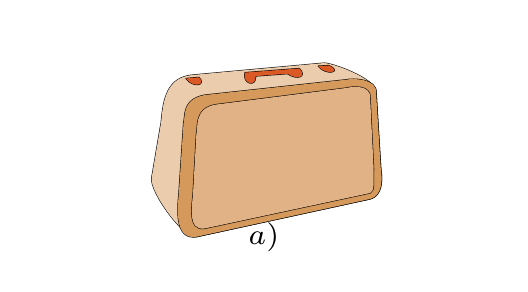
\begin{tikzpicture}[line join=round, line cap=round,scale=1.5,transform shape]
			\definecolor{bronze}{rgb}{0.8, 0.5, 0.2}
			\clip (-2,-1) rectangle (2,1);
			
			
			\tikzset{vali/.pic={
					\def\T0{
						%------------vien ngoai
						(-.6,.6)
						..controls +(-175:.22) and +(85:.2) ..  (-.87,.2)--(-.95,-.27)
						..controls +(-100:.12) and +(-160:.1) .. (-.57,-.77)--(.9,-.45)
						..controls +(15:.1) and +(-80:.1) .. (.99,-.2)--(.95,.45)
						..controls +(85:.12) and +(15:.05) .. (.5,.7)
						--cycle
						;}
					\draw \T0;
					\fill[bronze!40] \T0;
					\def\T1{
						%------------vien ngoai
						(-.5,.43)
						..controls +(-170:.2) and +(70:.05) ..  (-.68,.2)--(-.72,-.4)
						..controls +(-95:.1) and +(-170:.2) .. (-.57,-.77)--(.9,-.45)
						..controls +(15:.1) and +(-80:.1) .. (.99,-.2)--(.95,.45)
						..controls +(85:.12) and +(15:.05) .. (.7,.56)--cycle
						;}
					\draw \T1;
					\fill[bronze!80] \T1;
					\def\T2{
						%------------vien trong
						(-.4,.35)
						..controls +(-172:.2) and +(70:.05) ..  (-.572,.1)--(-.6,-.4)
						..controls +(-92:.07) and +(-170:.16) .. (-.5,-.7)--(.9,-.4)
						..controls +(25:.05) and +(-95:.1) .. (.93,-.2)--(.9,.4)
						..controls +(85:.12) and +(15:.05) .. (.7,.49)--cycle
						;}
					\draw \T2;
					\fill[bronze!60] \T2;
					\def\V{
						%------------vien ngoai
						(-.07,.59)
						..controls +(-85:.1) and +(-105:.1) ..  (-.16,.62)--(.3,.655)
						..controls +(-45:.1) and +(-35:.1) ..  (.2,.61)--cycle
						
						(-.55,.58)
						..controls +(-45:.1) and +(-55:.1) ..  (-.66,.57)--cycle
						
						(.55,.68)
						..controls +(-25:.14) and +(-55:.1) ..  (.46,.675)--cycle
						;}
					\draw \V;
					\fill[bronze!70!red] \V;
			}}
			
			\path(0,0)pic[scale=1]{vali}node[below,yshift=-15pt,,font=\scriptsize]{$a)$}; 	
		\end{tikzpicture}
		\begin{tikzpicture}[scale=0.7]
			\def\a{5}
			\path (	0,0) coordinate (D)--+(\a,0) coordinate (C)
			($(D)!0.1!60:(C)$) coordinate (x)
			($(D)!6!(x)$) coordinate (A)
			($(C)!0.1!-60:(D)$) coordinate (y)
			($(C)+(A)-(D)$) coordinate (x')
			(intersection of A--x' and C--y) coordinate (B)
			($(C)!(A)!(D)$) coordinate (E)
			;
			\path pic[draw,angle radius=5pt]{right angle=A--E--C};
			\draw (D)--(C)--(B)--(A)--cycle (A)--(E)
			;
			\foreach \t/\g in {D/-90,C/-90,A/90,B/90,E/-90}{
				\draw[fill=white] (\t) circle (1pt) node[shift={(\g:7pt)},font=\scriptsize]{$ \t $};
			}
			\node[below] at (current bounding box.south){$b)$};  	
		\end{tikzpicture}
	}
	\loigiai{
		\immini{
			Áp dụng định lí Pythagore vào $\triangle ADE$ vuông tại $E$, ta có
			\begin{eqnarray*}
				AD^2&=&AE^2+DE^2 \\
				DE^2&=&AD^2-AE^2=61^2-60^2=3721-3600=121=11^2\\
				DE&=&11\,\text{(cm)}.
			\end{eqnarray*}
			Kẻ $BF \perp CD$, khi đó $BF$ là đường cao của hình thang cân $ABCD$ nên $BF=60$ cm.\\
			Xét $\triangle ADE$ và $\triangle BCF$ có\\
			$\widehat{AED}=\widehat{BFC}=90^\circ$;\\
			$AD=BC$ (do $ABCD$ là hình thang cân);\\
			$\widehat{ADE}=\widehat{BCF}$ (do $ABCD$ là hình thang cân);\\
			Suy ra $ \triangle ADE=\triangle BCF$ (c.g.n).\\
			Suy ra $DE=CF=11$ cm (hai cạnh tương ứng).\\
			Mà $DE+EF+CF=DC$.\\
			Suy ra $EF=DC-DE-CF=92-11-11=70$ cm.\\
			Xét $\triangle ABE$ và $\triangle FEB$ có\\
			$\widehat{BAE}=\widehat{EFB}=90^\circ$;\\
			$BE$ là cạnh huyền chung;\\
			$\widehat{ABE}=\widehat{FEB}$ (hai góc so le trong do $AB \parallel CD$).\\
			Suy ra $\triangle ABE=\triangle FEB$ (cạnh huyền – góc nhọn).\\
			Suy ra $AB=EF=70$ cm (hai cạnh tương ứng).\\
			Vậy độ dài đáy nhỏ của hình thang cân là $70$ cm.
			
		}	
		{
			\begin{tikzpicture}[scale=0.7]
				\def\a{5}
				\path (	0,0) coordinate (D)--+(\a,0) coordinate (C)
				($(D)!0.1!60:(C)$) coordinate (x)
				($(D)!6!(x)$) coordinate (A)
				($(C)!0.1!-60:(D)$) coordinate (y)
				($(C)+(A)-(D)$) coordinate (x')
				(intersection of A--x' and C--y) coordinate (B)
				($(C)!(A)!(D)$) coordinate (E)
				($(C)!(B)!(D)$) coordinate (F)
				;
				\foreach \x/\y/\z in {A/E/C,B/F/C}{
					\path pic[draw,angle radius=5pt]{right angle=\x--\y--\z};
				}
				\draw (D)--(C)--(B)--(A)--cycle (A)--(E) (B)--(F)
				;
				\foreach \t/\g in {D/-90,C/-90,A/90,B/90,E/-90,F/-90}{
					\draw[fill=white] (\t) circle (1pt) node[shift={(\g:7pt)},font=\scriptsize]{$ \t $};
				}
			\end{tikzpicture}
		}
	}
\end{bt}
\begin{bt}%[9-EX-DeCuongToan9-L2-Nguyễn Tấn Tài]%[8H2V3-4]
	\immini{
	Một mặt tường của chân tháp cột cờ Hà Nội có dạng hình thang cân $ABCD$ (Hình vẽ). Cho biết $\widehat{D}=\widehat{C}=75^\circ$. Tìm số đo $\widehat{A}$ và $\widehat{B}$.
	}{
	\includegraphics[scale=0.15]{images/8C3-B3-1}
	}
	\loigiai{
		Hình thang cân $ABCD$ có $\widehat{D}=\widehat{C}=75^\circ$.\\
		Suy ra \\
		\begin{eqnarray*}
			\widehat{A}+\widehat{D}&=&180^\circ\\
			\widehat{A}+75^\circ&=&180^\circ\\
			\widehat{A}&=&180^\circ-75^\circ\\
			\widehat{A}&=&105^\circ.
		\end{eqnarray*}
		$\widehat{A}=\widehat{B}=180^\circ-75^\circ=105^\circ$.
	}
\end{bt}
%%=======Câu [số câu]=======%%
\begin{bt} %[9-EX-DeCuongToan9-L2-Nguyễn Tấn Tài]%[8H2V3-4]
	\immini{
	Một khung cửa sổ hình thang cân có chiều cao $3$ m, hai đáy là $3$ m và $1$ m. Tìm độ dài hai cạnh bên và hai đường chéo.
	}{
	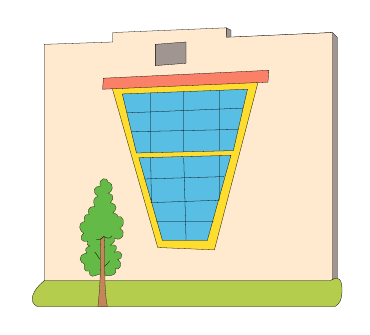
\begin{tikzpicture}[]
	\definecolor{xanhkinh}{RGB}{89,190,227}
	\definecolor{cam}{RGB}{250,128,104}
	\definecolor{vang}{RGB}{254,221,46}
	\definecolor{xam}{RGB}{161,149,145}
	\definecolor{xanhnen}{RGB}{180,205,76}
	\definecolor{hong}{RGB}{255,234,207}
	\definecolor{vien}{RGB}{40,34,11}
	\definecolor{nau}{RGB}{196,132,92}
	\definecolor{xanhcay}{RGB}{99,186,70}
	
	\filldraw[black,fill=xam,line width=0.1] (0.54,3.54) -- (0.6,3.51) -- (0.6,3.42) -- (1.89,3.48) -- (1.95,3.42) -- (1.95,0.09) -- (0.48,0.09) -- cycle;
	\filldraw[black,fill=hong,line width=0.1] (-1.77,0.09) -- (-1.77,3.33) -- (-0.9,3.36) -- (-0.9,3.48) -- (0.54,3.54) -- (0.54,3.42) -- (1.89,3.48) -- (1.89,0.09) -- cycle;
	\filldraw[black,fill=xam,line width=0.1] (-0.36,3.33) -- (-0.36,3.06) -- (0.03,3.09) -- (0.03,3.36) -- cycle;
	\filldraw[black,fill=vang,line width=0.1] (-0.33,0.75) -- (0.39,0.72) -- (0.96,2.91) -- (-0.93,2.85) -- cycle;
	\filldraw[black,fill=cam,line width=0.1] (-1.02,2.9) -- (1.08,3) -- (1.07,2.85) -- (-1.03,2.76) -- cycle;
	%Cửa sổ
	\filldraw[black,fill=xanhkinh,line width=0.1] (-0.78,2.7) -- (-0.6,1.95) -- (0.63,1.98) -- (0.81,2.76) -- cycle
	(-0.57,1.89) -- (-0.27,0.84) -- (0.3,0.84) -- (0.6,1.92) -- cycle;
	\draw[black,line width=0.1] 
	(-0.51,1.62) -- (0.51,1.65) 
	(0.38,1.08) -- (-0.35,1.08)
	(0,1.89) -- (0.03,0.84)
	(-0.42,1.89) -- (-0.41,1.32)
	(0.45,1.35)--(-0.42,1.32)
	(0.45,1.92) -- (0.45,1.35)
	
	(-0.66,2.22) -- (0.69,2.25)
	(-0.72,2.46) -- (0.75,2.52)
	(0,2.73) -- (0,1.97)
	(0.45,2.75) -- (0.45,1.98)
	(-0.42,2.71)--(-0.42,1.95)
	;
	\filldraw[black,fill=xanhnen,line cap=round,line join=round,line width=0.1] (-1.77,0.33) -- (1.86,0.33).. controls (2.01,0.42) and (2.01,0.27) .. (2.01,0.21).. controls (2.01,0.09) and (1.98,0.03) .. (1.92,0) -- (-1.86,0).. controls (-1.98,0.06) and (-1.92,0.21) .. (-1.77,0.33) -- cycle;
	\begin{scope}[shift={(-1.05,0)},scale=1,rotate=0]
		\filldraw[vien,fill=xanhcay,line width=0.1] (-0.03,0.41) -- (0.06,0.39).. controls (0.14,0.38) and (0.22,0.42) .. (0.18,0.48).. controls (0.22,0.45) and (0.3,0.54) .. (0.21,0.6).. controls (0.29,0.6) and (0.29,0.73) .. (0.17,0.69).. controls (0.22,0.75) and (0.2,0.8) .. (0.12,0.78).. controls (0.18,0.83) and (0.18,0.84) .. (0.17,0.87).. controls (0.27,0.81) and (0.33,0.95) .. (0.24,0.99).. controls (0.33,1.06) and (0.27,1.17) .. (0.21,1.14).. controls (0.21,1.19) and (0.18,1.17) .. (0.15,1.19).. controls (0.2,1.23) and (0.22,1.29) .. (0.12,1.32).. controls (0.18,1.4) and (0.15,1.42) .. (0.09,1.44).. controls (0.14,1.44) and (0.18,1.56) .. (0.09,1.58).. controls (0.09,1.65) and (-0.04,1.64) .. (-0.01,1.53).. controls (-0.09,1.53) and (-0.12,1.46) .. (-0.04,1.4).. controls (-0.09,1.38) and (-0.11,1.35) .. (-0.08,1.27).. controls (-0.18,1.27) and (-0.17,1.2) .. (-0.15,1.17).. controls (-0.2,1.17) and (-0.22,1.16) .. (-0.21,1.08).. controls (-0.32,1.05) and (-0.26,0.95) .. (-0.22,0.93).. controls (-0.29,0.87) and (-0.24,0.81) .. (-0.17,0.83).. controls (-0.18,0.8) and (-0.18,0.77) .. (-0.14,0.77).. controls (-0.2,0.75) and (-0.21,0.72) .. (-0.18,0.68).. controls (-0.32,0.65) and (-0.26,0.55) .. (-0.21,0.54).. controls (-0.22,0.51) and (-0.22,0.43) .. (-0.15,0.45).. controls (-0.15,0.35) and (-0.08,0.39) .. (-0.03,0.41) -- cycle;
		\filldraw[vien,fill=nau,line width=0.1] (-0.01,0.85) -- (0.04,0.89).. controls (0.06,0.54) and (0.03,0.26) .. (0.08,0) -- (-0.04,0).. controls (-0.01,0.27) and (0,0.55) .. (-0.01,0.84) -- cycle;
		\draw[vien,line width=0.15] (-0.01,0.6).. controls (-0.03,0.61) and (-0.06,0.68) .. (-0.08,0.69)
		(0.04,0.51).. controls (0.08,0.52) and (0.09,0.57) .. (0.11,0.58)
		(-0.06,0.85).. controls (-0.03,0.85) and (0,0.85) .. (0.03,0.89).. controls (0.08,0.87) and (0.11,0.85) .. (0.14,0.9)
		;
	\end{scope}
\end{tikzpicture}
	\begin{tikzpicture}[line join=round, line cap=round,font=\normalsize,>=stealth,scale=1]
		\path 
		(0,0) coordinate (A)
		(A)--++(100:3) coordinate (D)
		(A)--++(0:2.5) coordinate (B)
		(B)--++(80:3) coordinate (C)
		($(D)!(A)!(C)$) coordinate (H)
		($(D)!(B)!(C)$) coordinate (K)
		;
		\draw (A)--(B)--(C)--(D)--cycle (A)--(H) (B)--(K) (A)--(C) (B)--(D);
		\path (H) pic[draw,angle radius=5pt,angle eccentricity=2]{right angle=A--H--D};
		\path (K) pic[draw,angle radius=5pt,angle eccentricity=2]{right angle=B--K--C};
		\foreach \x/\g in {D/135,C/45,A/-90,B/-90,H/90,K/90}{
			\draw[fill=black] (\x) circle (0.05)+(\g:0.3) node {$\x$};
		};
	\end{tikzpicture}
	}
	\loigiai{
		Xét hình thang cân $ABCD$ ($AB \parallel DC$), đáy $AB=1$ m, đáy $DC=3$ m, chiều cao $3$ m. Kẻ $BK \perp DC$.\\
		Ta có $AB \parallel DC$ và $BK \perp DC$\\
		Suy ra $ BK \perp AB$.\\
		Xét $\triangle AHK$ và $\triangle ABK$ có\\
		$\widehat{KHA}=\widehat{ABK}=90^\circ$;\\
		$AK$ chung;\\
		$\widehat{AKH}=\widehat{KAB}$ (hai góc so le trong).\\
		Suy ra $\triangle AHK=\triangle ABK$ (cạnh huyền-góc nhọn).\\
		Suy ra $HK=BK=1$ m.\\
		Xét $\triangle AHD$ và $\triangle BKC$ có\\
		$\widehat{AHD}=\widehat{BKC}=90^\circ$;\\
		$\widehat{D}=\widehat{C}$ (vì hình thang cân);\\
		$AD=BC$ (tính chất hình thang cân).\\
		Suy ra $ \triangle AHD=\triangle BKC$ (cạnh huyền-góc nhọn).\\
		Suy ra $ DH=CK$ (hai cạnh tương ứng).\\
		Mà $DH+HK+CK=DC=3$ m.\\
		Suy ra $ 2DH=3-1=2$.\\
		Suy ra $ DH=1$ m.\\
		Suy ra $ HC=2$ m.\\
		Áp dụng định lý Py-ta-go trong $\triangle DAH$ vuông tại $H$\\
		$AD^2=AH^2+DH^2=3^2+1^2=9+1=10$\\
		$AD=\sqrt{10}$ (m).\\
		Suy ra $BC=\sqrt{10}$ m.\\
		Áp dụng định lý Py-ta-go trong $\triangle AHC$ vuông tại $H$\\
		$AC^2=AH^2+HC^2=3^2+2^2=9+4=13$\\
		$AC=\sqrt{13}$ m.\\
		Mà $BD=AC=\sqrt{13}$ m (do hình thang cân).
	}
\end{bt}
